\section{Implementation}

This pipeline was developed in MATLAB. Since the group consisted of four students, a Git repository was used to be able to work on different files simultaneously, and to enable version control.

\subsubsection{Coordinate Frames}
In this mini project the coordinate frames were defined as shown in \cref{img_coord_frames}. The camera coordinates are in a way oriented, that the x-y plane lies parallel to the image plane, while the z-axis is pointing towards the scenery. The world frame however is oriented in such a way that the x-y plane is parallel to the ground and the z-axis is pointing upwards. The origin of the world frame is at the same location as the origin of the first bootstrap image.

Transformation between frames are described by homogenous transformation matrices. $T_{AB}$ maps points from frame $B$ to frame $A$.

\begin{figure}[ht]
	\centering
	\includegraphics[width=0.5\textwidth]{impl/coord_frames}
	\caption{Coordinate Frames}
	\label{img_coord_frames}
\end{figure}

\subsubsection{Pipeline overview}
As shown in \cref{img_flow_rough} the pipeline consists of two parts:
\begin{compactenum}
	\item Bootstraping \& Initialization
	\item Continuous operation
\end{compactenum}

\begin{figure}[ht]
	\centering
	\includegraphics[width=0.5\textwidth]{impl/rough_chart}
	\caption{Overview flow chart}
	\label{img_flow_rough}
\end{figure}

\subsubsection{Conventions}
\begin{compactitem}
	\item Index of previous frame: $i$
	\item Index of current frame: $j$
	\item Index of frame for newly added candidate keypoint: $first$
	\item Pose difference between previous to current frame: $T_{C_iC_j}$
	\item $\left[u/v\right]$: Pixel coordinates
	\item Query keypoints: Keypoints newly generated in frame $j$ 
	\item Candidate keypoint: A keypoint without associated landmark
	\item Harris Matcher: Descriptor matching keypoint tracker (based on Harris features) developed during the lecture.
\end{compactitem}

\subsubsection{Options and parameters}
The pipeline was designed in a modular way. Key algorithms are abstracted into self-contained functions, as described in the pipeline overview. Next to this 'functional programming' approach all the tuning variables (e.g. number of keypoints, bearing angle thresholds, etc.) were centrally aggregated in a parameter struct.\\
For further insight please consult the function \code{loadParameters.m}.\\

In order to run the visual odometry two launch procedures where implemented:
\begin{compactitem}
	\item \textbf{Debug Mode:} For development and debug mode the main.m with default 		parameters can be executed. Numerous individual plots are displayed with insightful 		information about matching, inlier rejection and triangulation.
	\item \textbf{Simple GUI:} Out of performance reasons a more compact and user-friendly display of the pipeline output was created with a GUI designed with the Matlab GUIDE application, see figure \cref{img_gui}. Only the most crucial entities, like number of landmarks, are visualized for intuitive understanding.\\
\end {compactitem}

\textbf{How to run the GUI}
Please follow the steps below to run the visual odometry through the GUI environment:
\begin{compactenum}
	\item adapt dataset paths in \code{loadParameters.m}
	\item type into MATLAB command window: \code{gui\_simple}
	\item in \textit{Parameters} panel select dataset to run on and toggle respective radio buttons
	\item hit \textit{Run} to trigger the visual odometry\\
\end{compactenum}

Advanced parameter tuning can be achieved by changing the default parameters in \code{loadParameters.m}.

%\@ Miro please add pic of gui during operation
\begin{figure}[ht]
	\centering
	\includegraphics[width=\textwidth]{gui_nice}
	\captionsetup{justification=centering}
	\caption{Graphical user interface \\candidate keypoints (red $\bullet$), inlier keypoints (green $\bullet$), reprojected landmarks (green $\times$)}
	\label{img_gui}
\end{figure}


\subsubsection{Camera calibration}
Using the Camera Calibration Toolbox for Matlab\footnote{\url{www.vision.caltech.edu/bouguetj/calib_doc/}} from Jean-Yves Bouguet (Caltech) the camera of the an iphone 7 Plus was calibrated. A set of 17 calibration images where extracted from a calibration sequence filming a checker-board pattern from various angles.

\begin{figure}[htbp]
	\centering
	\begin{minipage}{0.4\textwidth} 
		\centering
		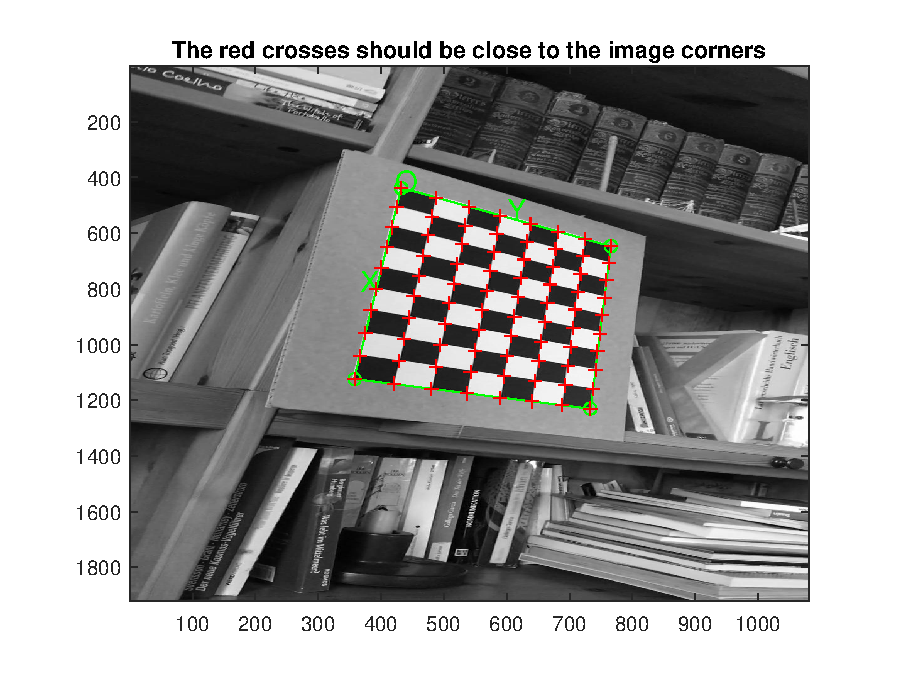
\includegraphics[width=0.9\textwidth]{impl/calibration_image_iphone7}
		\caption{Calibration pattern coordinate system aligned after corner selection}
		\label{img_calib}
	\end{minipage}
	%\hfill	
	\begin{minipage}{0.4\textwidth}
		\centering
		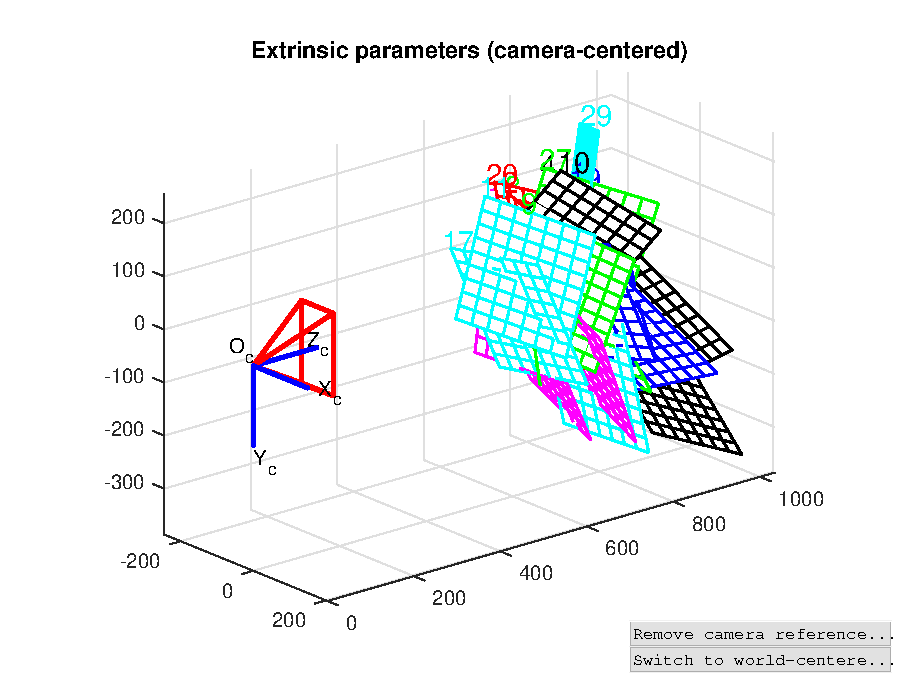
\includegraphics[width=0.9\textwidth]{impl/extrinsics}
		\caption{Relative to camera pattern poses}
		\label{img_calib} 
	\end{minipage}
\end{figure}

The camera intrinsics parameters together with a fourth-order polynomial approximation of the radial-tangential distortion were calculated based on the assumption of the skew being zero. The exact values and error margins are to be found on the Github repository.\\

Given these calibration parameters the VO pipeline was also applied on self-generated datasets called \textit{Poly-Up} and \textit{Poly-Down}. Note, that no undistortion was performed, since testing showed it to be negligible.

\subsection{Initialization}
\label{sec_init}

\subsubsection{Bootstraping}

\subsubsection{? findCorrespondences}

\subsubsection{eightPointRansac}

\subsubsection{linearTriangulation}
maybe only 1 sentences - ``like in the exercise''

\subsubsection{bundleAdjust}
is here anything different then in the continuous bundle adjust?

\subsubsection{applySphericalFilter}
have a look at \cref{triang_cont}. Maybe put this up to here and make a cref there.

\begin{figure}[ht]
	\centering
	\includegraphics[width=0.8\textwidth]{init_chart}
	\caption{Init Flow chart}
	\label{img_flow_init}
\end{figure}
\clearpage{\pagestyle{plain}\cleardoublepage}
\subsection{Continuous Operation}
\label{sec_cont_op}
Continuous operation of the VO pipeline is implemented in the 'process frame' function. It tracks keypoints with corresponding landmarks over several frames while estimating the pose difference between successive frames. Further, a keypoint tracker finds new candidate keypoints which will become new landmarks if a candidate keypoint was tracked far enough and achieved 'good' trianguability. This ensures to never run out of landmarks and keypoints if the image changes over time. The routines of the continuous operation shown in \cref{img_flow_cont} are described below.

\begin{figure}[ht]
	\centering
	\includegraphics[width=0.6\textwidth]{cont/cont_chart}
	\caption{Continuous operation flow chart}
	\label{img_flow_cont}
\end{figure}

\subsubsection{Relative pose estimation}
\label{ransac_cont}
To estimate the pose difference $T_{C_iC_j}$ from frame $i$ to $j$ we use the p3p-RANSAC algorithm also used in exercise 5. If wished the RANSAC can also use DLT pose estimation. Using these RANSAC algorithm ensures to remove outliers from our landmarks. We don't use DLT refinement after the p3p RANSAC since the best guess from p3p often gave better results.

\subsubsection{find\_correspondences\_cont()}
Tracking keypoints with existing landmarks from frame $i$ to frame $j$ is achieved by the function $find\_correspondences\_cont$. The user can choose whether to use a KLT or Harris matcher. As a by-product, the generated query keypoints are saved to be used by the candidate keypoint tracker in a successive step so they don't have to be generated twice which saves computation time. The number of generated query keypoints is adjustable by a parameter. In case the KLT tracker is active (which does not return query keypoints by default) new query keypoints are generated using Harris features. The amount of newly generated keypoints is the difference of remaining and wished candidate keypoints.

\subsubsection{updateKpTracks()}
In every frame, candidate keypoints from previous frames are tracked to $j$-frame. Every candidate keypoint track consists of the following entries: $\left\{\left[u/v\right]_j, \left[u/v\right]_{first}, T_{WC_{first}}, nr\_trackings\right\}$. After successive tracking, $[u/v]_j$ as well as the number of successful successive trackings are updated. The user can choose whether to use a KLT or a Harris matcher.
In case a candidate keypoint could not be tracked it's whole track gets removed from the tracker. If there are less candidate keypoints in the tracker then desired, newly generated keypoints (generated in find\_correspondences\_cont) are added to the tracker. Every newly added keypoint is stored together with the current pose $T_{WC_{first}}$.

\subsubsection{triangulateNewLandmarks()}
\label{triang_cont}
In order to localize correctly (see \cref{ransac_cont}), a sufficient number of landmarks is required. If the number of landmarks in the current frame drops below a certain threshold, the 'triangulateNewLandmarks' function is called to generate new landmarks from the candidate keypoint tracks. To check, whether a candidate keypoint is ready for triangulation the bearing angle between it's first and it's current observation is calculated. This is done for every keypoint candidate. If the bearing angle of a candidate keypoint exceeds a certain threshold, it is removed from the keypoint tracker and a new landmark gets triangulated with the algorithm developed in exercise 4.\\
\textbf{Adaptive bearing angle threshold: }The bearing angle threshold is adaptive to the number of remaining landmarks. The higher the number of remaining landmarks the higher the threshold. This ensures generation of new landmarks in case the filter starts to run out of landmarks but improves triangulation results once enough landmarks are in the pipeline. See also parameter 'increase bearing angle threshold' in \cref{params_table}.\\
\textbf{Filters:} Two filters are implemented to discard outliers within the newly generated landmarks (e.g. from image noise):
\begin{compactenum}
	\item Spherical filter: Already described in \cref{sub_sec_sphFilter}.
	\item Reprojected error filter: Landmarks passed the spherical filter get reprojected into the current frame. If the reprojected point is too far apart from the candidate keypoint coordinates it is discarded.
\end{compactenum}
Landmarks and their corresponding keypoints which passed these two filters are appended to the existing landmarks and keypoints vectors and will be used during the next localization iteration.

\subsubsection{Bundle Adjustment}
\textcolor[rgb]{1,0,0}{Todo: @Miro}
Explain how it works - add to flowchart

\subsubsection{Reinitialization}
The quality of the transformation matrix estimated by the p3p-RANSAC depends on the number of inlier landmarks. If there are enough inlier landmarks, the pose found by the p3p-RANSAC is a good estimation. However, if there are too few inlier landmarks, the estimated pose can be considered as too inaccurate for a further use. The fact that too few landmarks were found is a sign that the last few poses weren't good enough. It is therefore a good idea to discard some of the previous poses. The reinitialization discards the last \begin{math} n \end{math} poses and reinitializes the pipeline with the current image\begin{math} j \end{math} and the image \begin{math} j-(n+1) \end{math}.
\clearpage{\pagestyle{plain}\cleardoublepage}